\documentclass[12pt,twoside]{report}
\usepackage[utf8]{inputenc}
\usepackage{graphicx}
\graphicspath{ {images/} }
\usepackage{caption}
\usepackage{subcaption}
\usepackage[a4paper,width=150mm,top=25mm,bottom=25mm,bindingoffset=6mm]{geometry}
\usepackage{fancyhdr}
\usepackage{listings}
\usepackage{hyperref}
\usepackage{amsfonts}
\usepackage{amssymb}

\pagestyle{fancy}
\fancyhead{}
\fancyhead[RO,LE]{Machine Learning
for simulated control tasks with Webots}
\fancyfoot{}
\fancyfoot[LE,RO]{\thepage}
\fancyfoot[LO,CE]{Chapter \thechapter}
\fancyfoot[CO,RE]{Joan Gerard}
\renewcommand{\headrulewidth}{0.4pt}
\renewcommand{\footrulewidth}{0.4pt}

%%%%%%%%%%%%%%%%%%%%%%%%%%%%%%%
% CODE STYLE CONFIG
%%%%%%%%%%%%%%%%%%%%%%%%%%%%%%%
\usepackage{color}
\definecolor{codegreen}{rgb}{0,0.6,0}
\definecolor{codegray}{rgb}{0.5,0.5,0.5}
\definecolor{codepurple}{rgb}{0.58,0,0.82}
\definecolor{backcolour}{rgb}{0.95,0.95,0.92}
 
\lstdefinestyle{mystyle}{
    backgroundcolor=\color{backcolour},   
    commentstyle=\color{codegreen},
    keywordstyle=\color{magenta},
    numberstyle=\tiny\color{codegray},
    stringstyle=\color{codepurple},
    basicstyle=\footnotesize,
    breakatwhitespace=false,         
    breaklines=true,                 
    captionpos=b,                    
    keepspaces=true,                 
    numbers=left,                    
    numbersep=5pt,                  
    showspaces=false,                
    showstringspaces=false,
    showtabs=false,                  
    tabsize=2,
    aboveskip=20pt,
    belowskip=15pt
}
 
\lstset{style=mystyle}

%%%%%%%%%%%%%%%%%%%%%%%%%%%%%%%
% IMAGES PATH
%%%%%%%%%%%%%%%%%%%%%%%%%%%%%%%
\newcommand{\images}{images/}

%%%%%%%%%%%%%%%%%%%%%%%%%%%%%%%
% PARAGRAPH SEPARATION
%%%%%%%%%%%%%%%%%%%%%%%%%%%%%%%
\setlength{\parskip}{\baselineskip}
\setlength{\parindent}{0pt}

%%%%%%%%%%%%%%%%%%%%%%%%%%%%%%% 
% BIBLIOGRAPHIC REFERENCES
%%%%%%%%%%%%%%%%%%%%%%%%%%%%%%%
\usepackage[sorting=none]{biblatex}
\addbibresource{references.bib}

\title{Preparatory work for the Master Thesis}
\author{Joan Gerard}
\date{Academic year 2019}

\newcommand{\source}[1]{
	\vspace{-3pt}
	\caption*{ \textbf{Source}: {#1}} 
}

\begin{document}

\begin{titlepage}
    \begin{center}
        
        \normalsize
        \textbf{UNIVERSITÉ LIBRE DE BRUXELLES}\\
        \small
        \textbf{Faculté de Sciences}\\
        \textbf{Département d'Informatique}\\
        
        \vspace{4.0cm}
        \huge
        Preparatory work for the Master Thesis\\
        \vspace{0.5cm}
        \Huge
        Machine Learning\\
        for Probabilistic Robotics\\
        with Webots\\
        
        \vspace{0.5cm}
        \normalsize
        Joan Gerard
        
        \vspace{7cm}
        \small
        \textbf{Promotor:} Prof. Gianluca Bontempi
        
        \vspace{4cm}
        \footnotesize
         \textbf{Academic year 2019}
        
    \end{center}
\end{titlepage}

%\thispagestyle{plain}
\begin{center}
    \Large
    \textbf{Thesis Title}
    
    \vspace{0.4cm}
    \large
    Thesis Subtitle
    
    \vspace{0.4cm}
    \textbf{Author Name}
    
    \vspace{0.9cm}
    \textbf{Abstract}
\end{center}
Lorem ipsum dolor sit amet, consectetur adipisicing elit, sed do eiusmod tempor incididunt ut labore et dolore magna aliqua. Ut enim ad minim veniam, quis nostrud exercitation ullamco laboris nisi ut aliquip ex ea commodo consequat. Duis aute irure dolor in reprehenderit in voluptate velit esse cillum dolore eu fugiat nulla pariatur. Excepteur sint occaecat cupidatat non proident, sunt in culpa qui officia deserunt mollit anim id est laborum.

Lorem ipsum dolor sit amet, consectetur adipisicing elit, sed do eiusmod tempor incididunt ut labore et dolore magna aliqua. Ut enim ad minim veniam, quis nostrud exercitation ullamco laboris nisi ut aliquip ex ea commodo consequat. Duis aute irure dolor in reprehenderit in voluptate velit esse cillum dolore eu fugiat nulla pariatur. Excepteur sint occaecat cupidatat non proident, sunt in culpa qui officia deserunt mollit anim id est laborum.

Lorem ipsum dolor sit amet, consectetur adipisicing elit, sed do eiusmod tempor incididunt ut labore et dolore magna aliqua. Ut enim ad minim veniam, quis nostrud exercitation ullamco laboris nisi ut aliquip ex ea commodo consequat. Duis aute irure dolor in reprehenderit in voluptate velit esse cillum dolore eu fugiat nulla pariatur. Excepteur sint occaecat cupidatat non proident, sunt in culpa qui officia deserunt mollit anim id est laborum.

\tableofcontents

\listoffigures

\listoftables

\chapter{Introduction}
Lorem ipsum dolor sit amet, consectetur adipisicing elit, sed do eiusmod tempor incididunt ut labore et dolore magna aliqua. Ut enim ad minim veniam, quis nostrud exercitation ullamco laboris nisi ut aliquip ex ea commodo consequat. Duis aute irure dolor in reprehenderit in voluptate velit esse cillum dolore eu fugiat nulla pariatur. Excepteur sint occaecat cupidatat non proident, sunt in culpa qui officia deserunt mollit anim id est laborum.

Lorem ipsum dolor sit amet, consectetur adipisicing elit, sed do eiusmod tempor incididunt ut labore et dolore magna aliqua. Ut enim ad minim veniam, quis nostrud exercitation ullamco laboris nisi ut aliquip ex ea commodo consequat. Duis aute irure dolor in reprehenderit in voluptate velit esse cillum dolore eu fugiat nulla pariatur. Excepteur sint occaecat cupidatat non proident, sunt in culpa qui officia deserunt mollit anim id est laborum.

Lorem ipsum dolor sit amet, consectetur adipisicing elit, sed do eiusmod tempor incididunt ut labore et dolore magna aliqua. Ut enim ad minim veniam, quis nostrud exercitation ullamco laboris nisi ut aliquip ex ea commodo consequat. Duis aute irure dolor in reprehenderit in voluptate velit esse cillum dolore eu fugiat nulla pariatur. Excepteur sint occaecat cupidatat non proident, sunt in culpa qui officia deserunt mollit anim id est laborum.

Lorem ipsum dolor sit amet, consectetur adipisicing elit, sed do eiusmod tempor incididunt ut labore et dolore magna aliqua. Ut enim ad minim veniam, quis nostrud exercitation ullamco laboris nisi ut aliquip ex ea commodo consequat. Duis aute irure dolor in reprehenderit in voluptate velit esse cillum dolore eu fugiat nulla pariatur. Excepteur sint occaecat cupidatat non proident, sunt in culpa qui officia deserunt mollit anim id est laborum.

Lorem ipsum dolor sit amet, consectetur adipisicing elit, sed do eiusmod tempor incididunt ut labore et dolore magna aliqua. Ut enim ad minim veniam, quis nostrud exercitation ullamco laboris nisi ut aliquip ex ea commodo consequat. Duis aute irure dolor in reprehenderit in voluptate velit esse cillum dolore eu fugiat nulla pariatur. Excepteur sint occaecat cupidatat non proident, sunt in culpa qui officia deserunt mollit anim id est laborum.

Lorem ipsum dolor sit amet, consectetur adipisicing elit, sed do eiusmod tempor incididunt ut labore et dolore magna aliqua. Ut enim ad minim veniam, quis nostrud exercitation ullamco laboris nisi ut aliquip ex ea commodo consequat. Duis aute irure dolor in reprehenderit in voluptate velit esse cillum dolore eu fugiat nulla pariatur. Excepteur sint occaecat cupidatat non proident, sunt in culpa qui officia deserunt mollit anim id est laborum.

\chapter{State of the art}
\section{Webots}
Webots was created by Cyberbotics Ltd. a spin-off company from the EPFL and has been developing it since 1998. It currently\footnote{2019} employs 6 people in Lausanne, Switzerland to continuously develop Webots according to customers needs. Cyberbotics provides consulting on both industrial and academic research projects and delivers open-source software solutions to its customers. It also provides user support and training to the users of the Webots software. The source code and binary packages are available for free; however, user support and consultancy are not. It is available for Windows, Ubuntu Linux and MacOS \cite{cyberbotics}.

Webots website has a reference manual that describes nodes and API functions. It has a complete user guide as well endowed with examples of simulations that show the use of actuators, creation of different environments, geometries primitives, complex behaviors, functionalities and advanced 3D rendering capabilities. This section is oriented to describe the basics of Webots and it is focused on what will be useful to develop the project. For a detailed description please refer to the user guide\footnote{\url{https://cyberbotics.com/doc/guide/index}} or the reference manual\footnote{\url{https://cyberbotics.com/doc/reference/index}}.

\subsection{Graphic Interface}
Webots supports the following programming languages: C, C++, Python, Java, MATLAB and ROS. Additionally, it offers the possibility of creating a custom interface to third-party software such as Lisp\textsuperscript{TM} or LabView\textsuperscript{TM} using TCP/IP protocol.

\begin{figure}[h]
	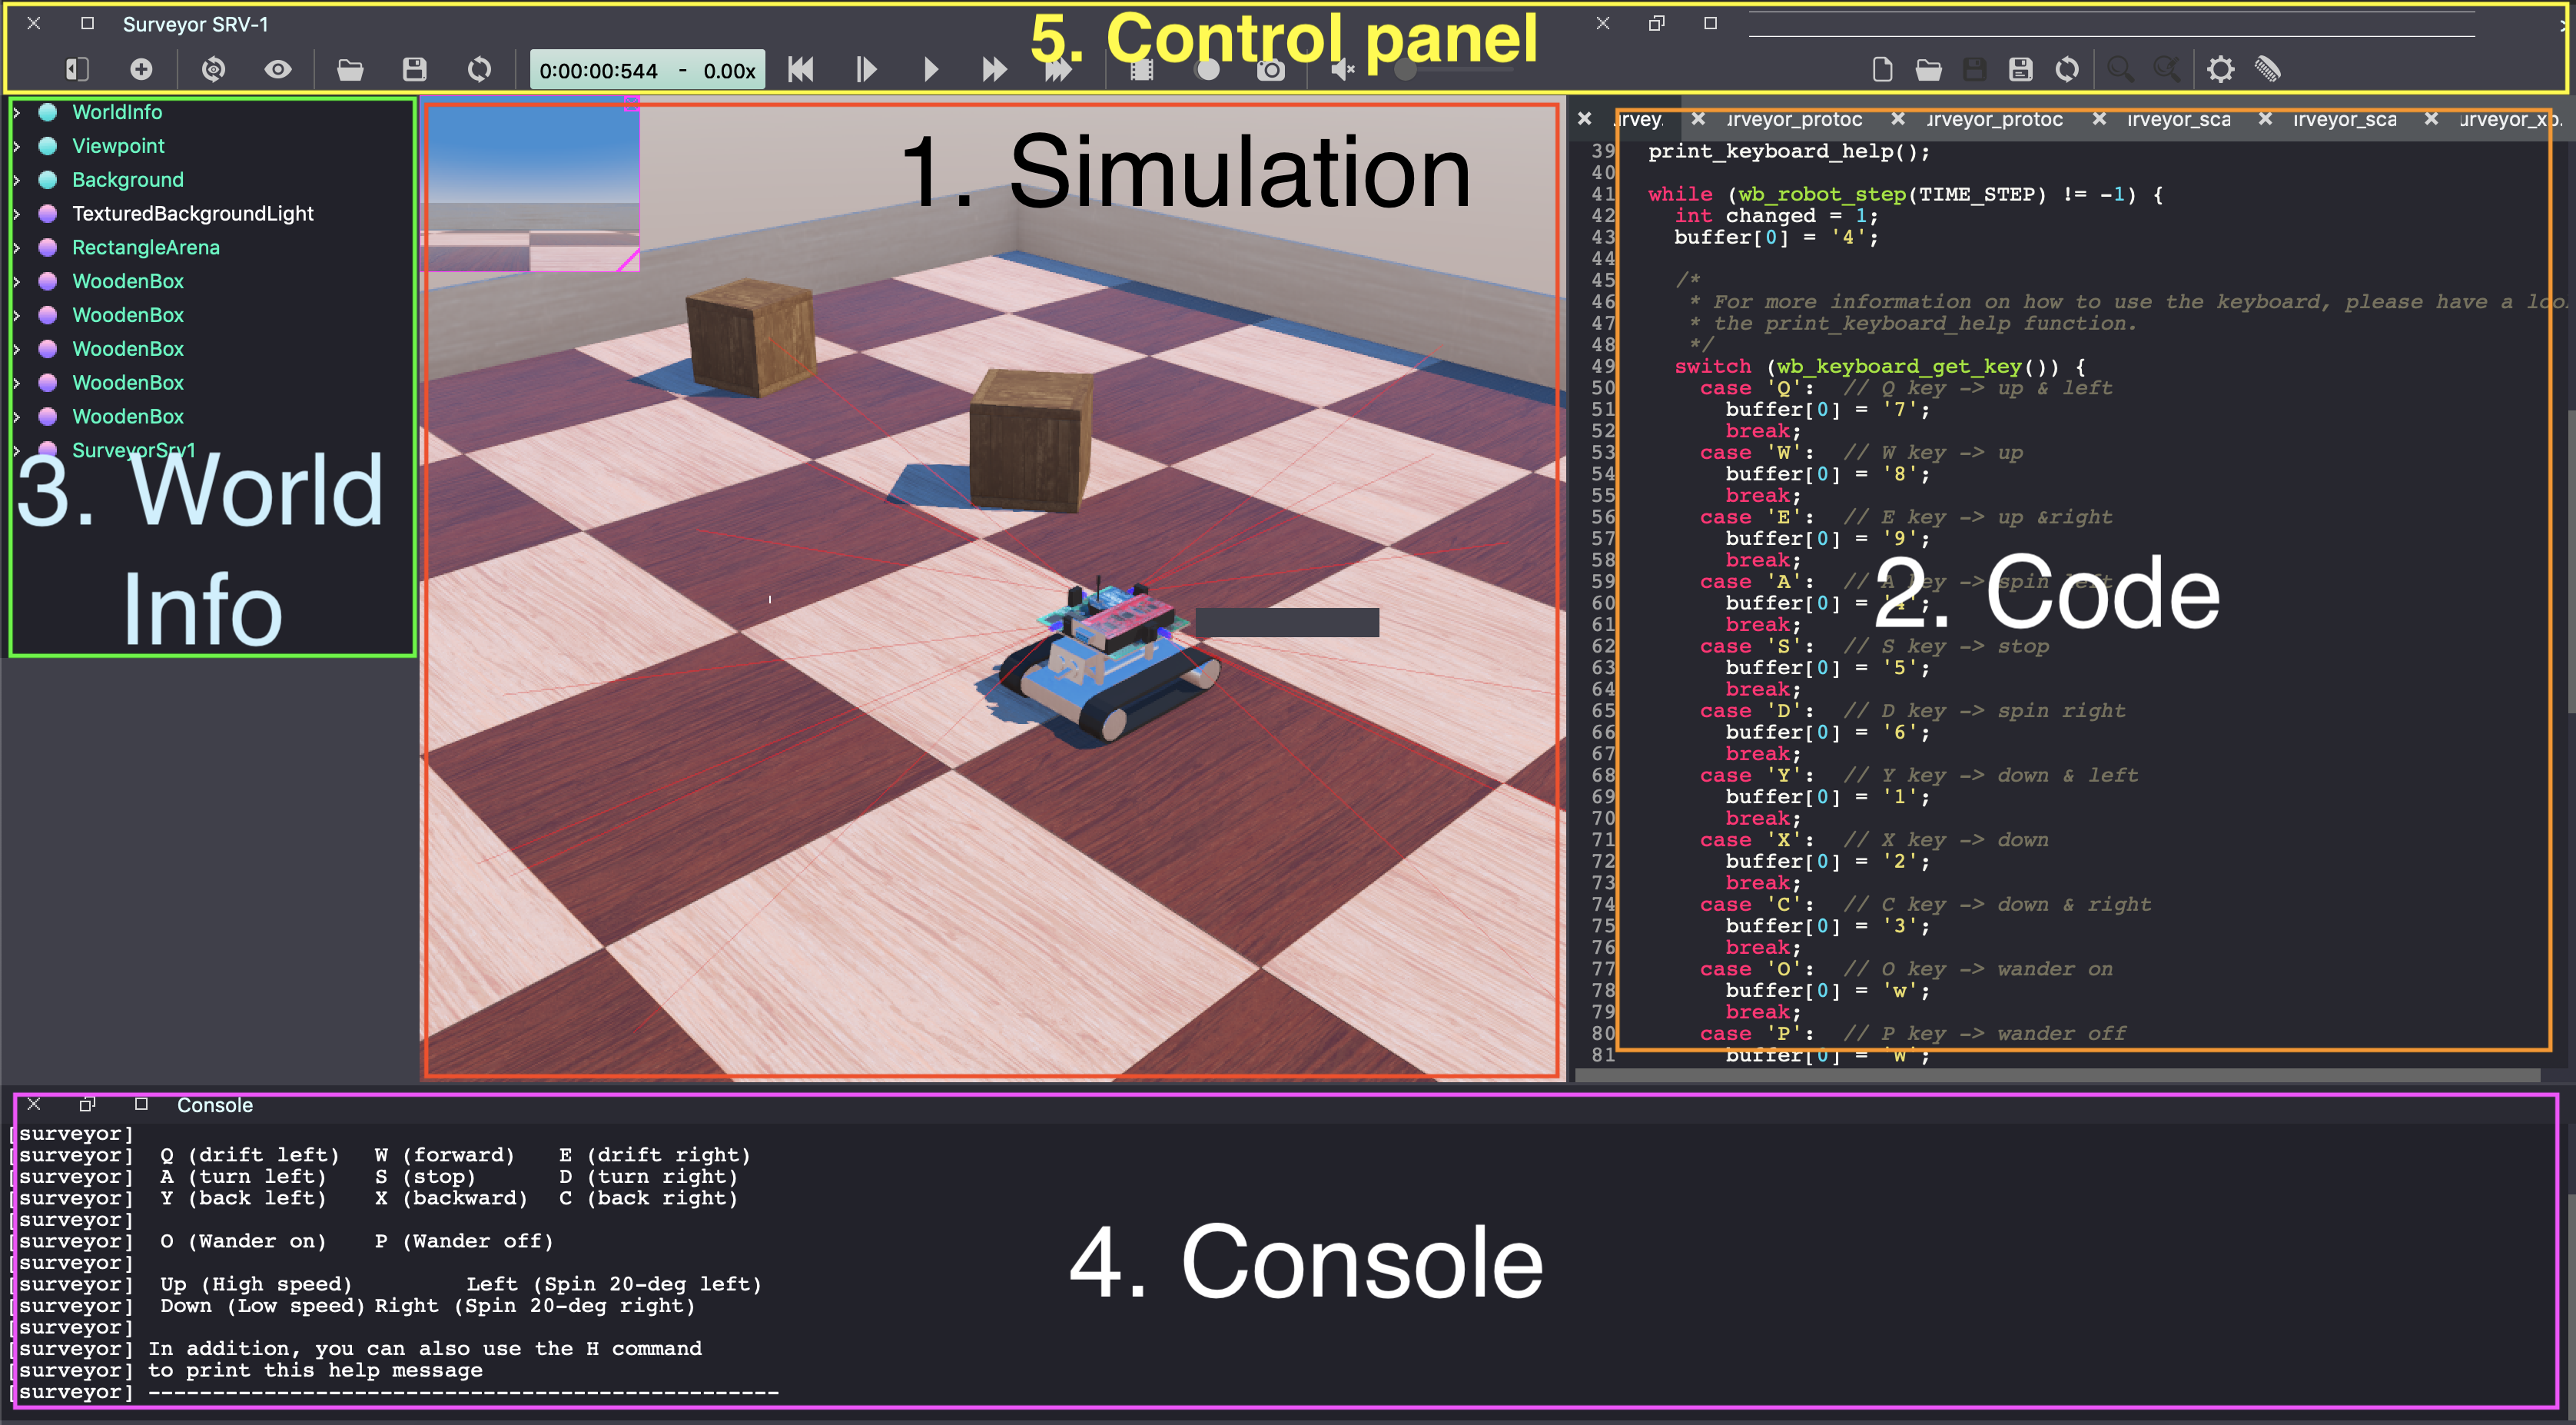
\includegraphics[width=\linewidth]{\images/chapter2/interface.png}
	\caption{Webots graphic interface}
	\label{fig-ch-2:interface}
\end{figure}

Figure \ref{fig-ch-2:interface} shows the main graphic interface of Webots. It can be divided in 5 panels:

\begin{enumerate}
	\item Simulation: graphic visualization of the simulated world objects.
	\item Code visualization: robot controller code editor.
	\item World Information: information about the simulated world.
	\item Console: program execution output stream.
	\item Control panel: set of buttons that controls the simulation execution.
\end{enumerate}

The program allows users to create highly personalized simulated environments which are called worlds, from scratch using pre-built 3D object models such as robots, wood boxes, walls, arenas, etc. A robot needs to be associated with a controller program that contains the source code with the desired behavior. This controller can be easily edited in the code panel and once it is saved it is automatically reloaded into all the robots associated with it. For running the simulation users can play, stop or reset it, among other options, using the control panel set of buttons. The output stream of the controller execution will be displayed in the console panel. 


\subsection{Webots with Python 3.7 and TensorFlow}

Python was created in 1990 by Guido van Rossum at Stichting Mathematisch Centrum in the Netherlands as a successor of a language called ABC\cite{python-docs}. Nowadays it has became one of the most popular programming languages for data science\cite{Raschka:2015:PML:2886323}.

The Python API of Webots was created from C++ API and it supports Python 3.7. It is possible to configure Webots to use Python 3.7 which should be previously installed from the Python website\footnote{Download it from \url{https://www.python.org}}; however, Webots does not work properly with Python versions installed from package managers as Brew. By default Webots is configured to use the default installed version of Python. In order to use another version, access to the menu options in Webots: \path{Webots/Preferences}; the \textit{Python command} label should point out to the installation path of Python3.7 as it is shown in figure \ref{fig-ch-2:python}. 

\begin{figure}[ht]
	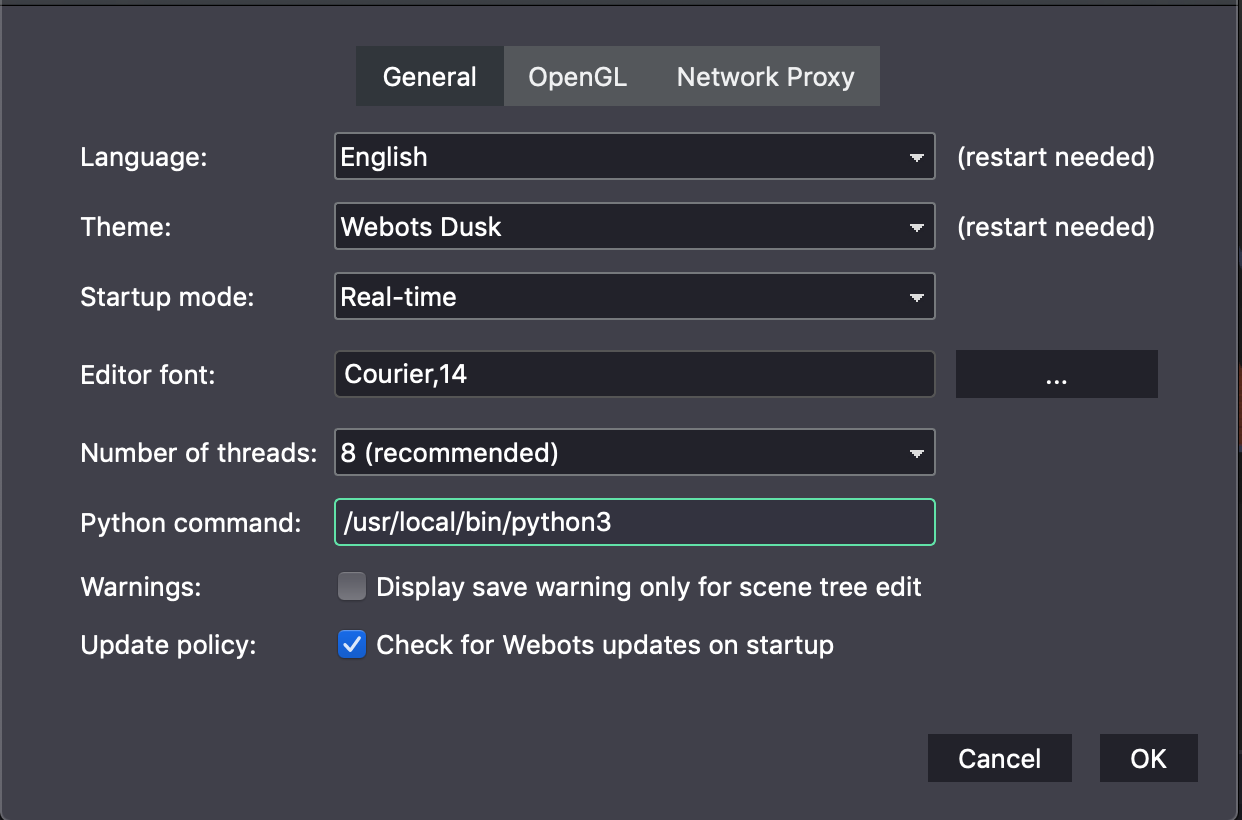
\includegraphics[width=\linewidth]{\images/chapter2/preferences.png}
	\caption{Configure Python3.7}
	\label{fig-ch-2:python}
\end{figure}

Python allows to install third-party libraries like TensorFlow which is a Python-friendly open-source library developed by the researchers and engineers of the Google Brain team for internal use only and  then released in November 2015 under a permissive open source license. It implements machine learning algorithms and deep learning wrappers\cite{Raschka:2015:PML:2886323}.

The \verb|pip3| command allows to install any library for Python 3.7. For installing TensorFlow type \verb|pip3 install tensorflow| in the console terminal. For verifying the correct installation, the code displayed in listing \ref{code:verify-tf} can be put inside a controller application in Webots.

\begin{lstlisting}[language=Python, caption=Verify correct installation of TensorFlow, label=code:verify-tf]
import tensorflow as tf

verifier = tf.constant('TensorFlow was installed correctly.')
sess = tf.Session()
print(sess.run(verifier))
\end{lstlisting}

If TensorFlow was correctly installed, after the execution of the simulation, a message in the console panel will be displayed informing about its correct installation.


\subsection{Robots and world creation}

Webots allows creating large simulated worlds. The world description and content is presented as a tree structure where each node represents an object in the world, those objects have themselves nodes and sub-nodes within a name and a value indicating different physical characteristics or components. 

\begin{figure}[h!]
  \centering
  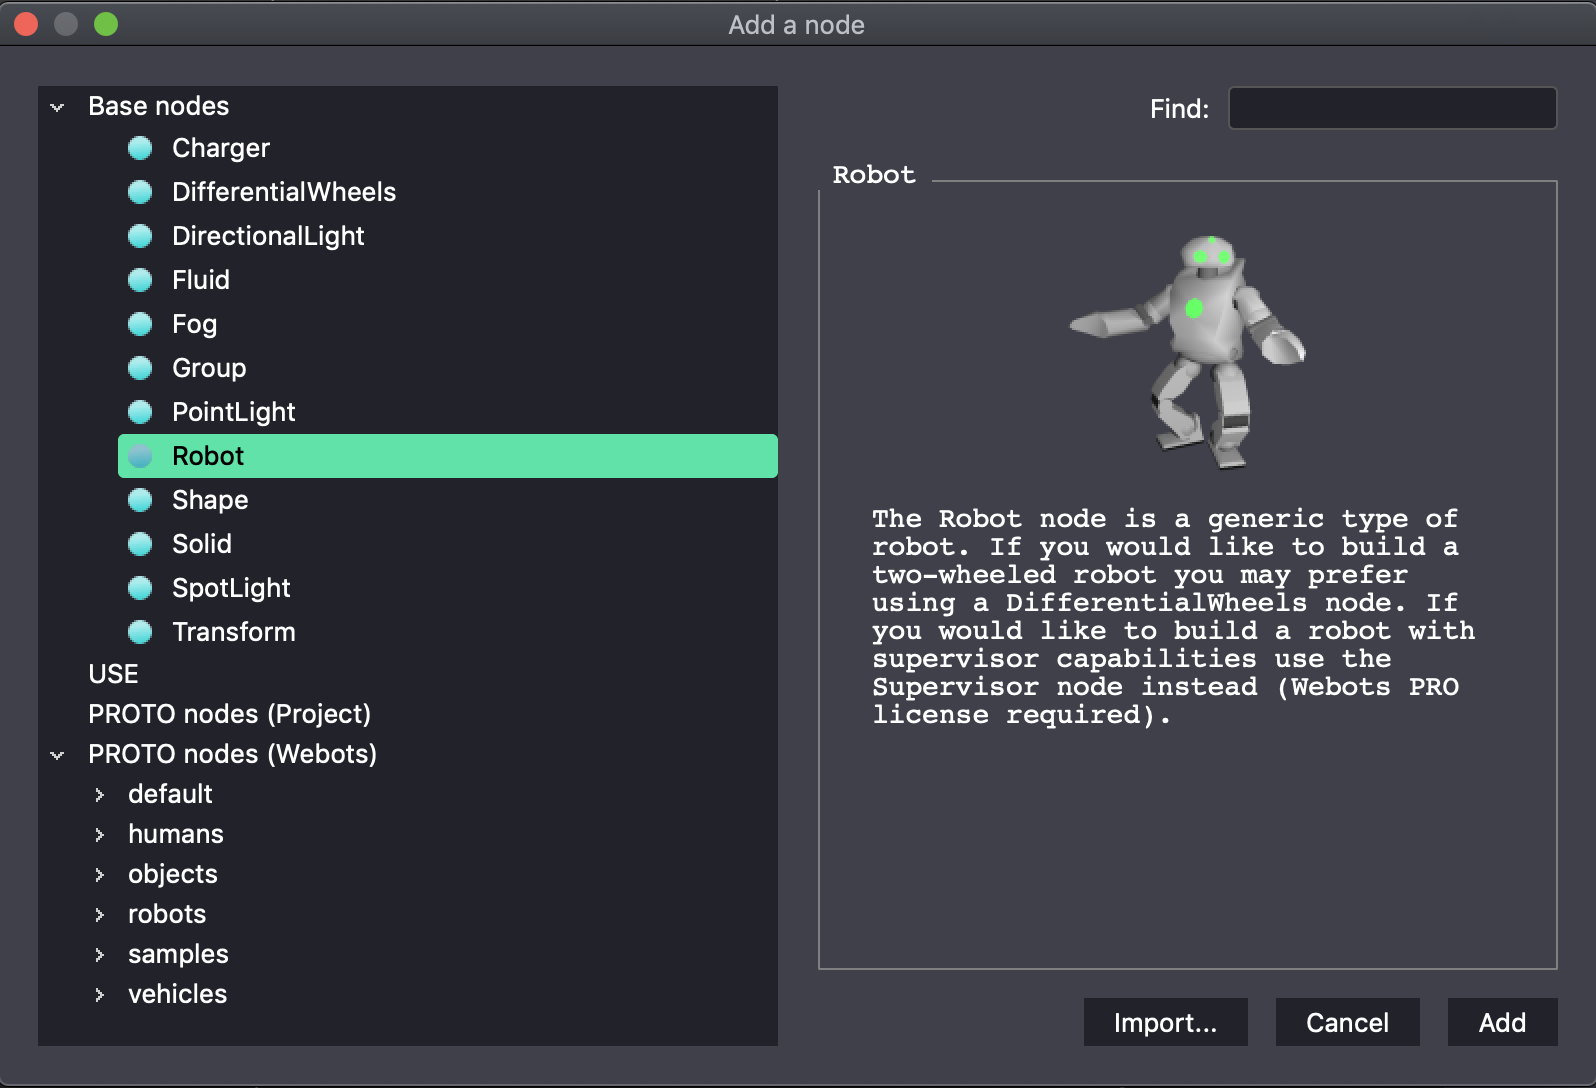
\includegraphics[width=0.8\linewidth]{\images/chapter2/nodes.png}
  \caption{World structure}
  \label{fig:ch-2:nodes}
\end{figure}

For adding a node into the world we can press the \verb|Add object| button that will open the window shown in figure \ref{fig:ch-2:nodes}. The base nodes are the basic objects that can be part of the world. Moreover, they are simpler models than the others. The USE nodes are objects that were already created in the world and can be reused. For instance, if a wood box was added into the world with some specific physical characteristics, a name can be assigned to its USE attribute and then it can be reused instead of creating a new one with same characteristics. The PROTO nodes contains a set of 3D models as robots, objects, vehicles, etc. Fruits, toys, drinks, plants, chairs, stairs and buildings are only a small part of the big set of modeled objects. The robots node offers as well a big diversity of models. From simple robots as the e-puck (figure \ref{fig:ch-2:e-puck}) model which is used very often in research, to more complex robots as the very well known humanoid Nao (figure \ref{fig:ch-2:nao}) are some examples of a total of 44 3D modeled robots that are available to use within the simulator tool. 

\begin{figure}[h!]
  \centering
  \begin{subfigure}[b]{0.3\linewidth}
  	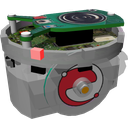
\includegraphics[width=\linewidth]{\images/chapter2/e-puck.png}
  	\caption{e-puck}
  	\label{fig:ch-2:e-puck}
  \end{subfigure}
  \begin{subfigure}[b]{0.35\linewidth}
  	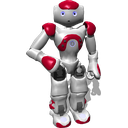
\includegraphics[width=\linewidth]{\images/chapter2/nao.png}
  	\caption{Nao}
  	\label{fig:ch-2:nao}
  \end{subfigure}
  \caption{Robots}
\end{figure}

Another powerful feature of Webots is to create a custom robot model from scratch using a tree-based structure of solid nodes which are virtual objects with physical properties. Thus a robot is made of a set of solid nodes put them together using joint nodes which are abstract nodes that models mechanical joints. Figure \ref{fig:ch-2:joints} shows the different types of joints that can be used.

\begin{figure}[h!]
  \centering
  \begin{subfigure}[b]{0.47\linewidth}
  	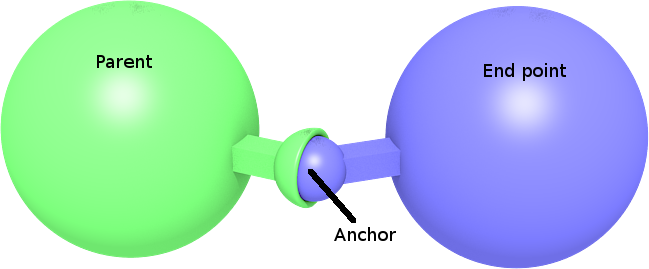
\includegraphics[width=\linewidth]{\images/chapter2/ballJoint.png}
  	\caption{Ball Joint}
  	\label{fig:ch-2:ball-joint}
  \end{subfigure}
  \vspace{0.00mm}
  \begin{subfigure}[b]{0.47\linewidth}
  	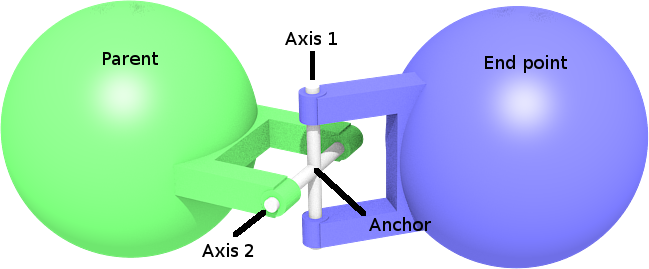
\includegraphics[width=\linewidth]{\images/chapter2/hinge2Joint.png}
  	\caption{Hinge 2 Joint}
  	\label{fig:ch-2:highe-2-joint}
  \end{subfigure}
  \vspace{0.00mm}
  \begin{subfigure}[b]{0.47\linewidth}
  	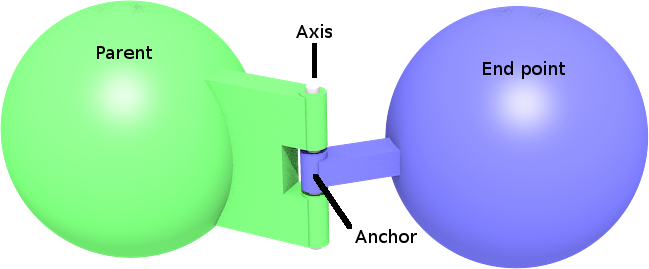
\includegraphics[width=\linewidth]{\images/chapter2/hingeJoint.png}
  	\caption{Hinge Joint}
  	\label{fig:ch-2:hinge-joint}
  \end{subfigure}
  \vspace{0.00mm}
  \begin{subfigure}[b]{0.47\linewidth}
  	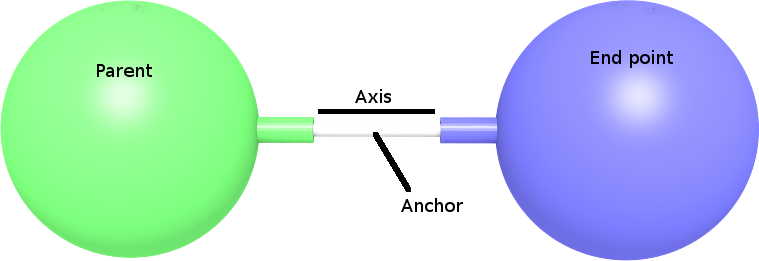
\includegraphics[width=\linewidth]{\images/chapter2/sliderJoint.png}
  	\caption{Slider Joint}
  	\label{fig:ch-2:slider-joint}
  \end{subfigure}
  \caption{Different types of joint nodes}
  \source{Webots documentation}
  \label{fig:ch-2:joints}
\end{figure}


A position sensor can be added into the devices property of a joint node in order to monitor it. In like manner a rotational motor node can be added for actuating it. Thus, putting all together a simplistic version of a custom robot can be created based on the tree information and properties given to the simulator.

\subsection{Sensors}

Sensors allows the robot to sense the environment. Webots has a wide range of generic and commercially available sensors that can be plugged into a custom robot. On one side, the compass, distance sensor and position sensor are some few examples of generic sensors. On the other side, camera, lidar, radar and range finder sensors built by different manufacturers as Hokuyo, Velodyne and Microsoft are offered as subcategories of commercially available sensors. 

\begin{itemize}
\item{The \textbf{compass sensor} can be used to express the position of the virtual north as a 1, 2 or 3-axis vector in relation to the position of the robot. The virtual north can be specified in the WorldInfo node by the \verb|northDirection| field. The major fields that can be customized are: the xAxis, yAxis, zAxis, lookup table and resolution field. }
\item{The \textbf{distance sensor} measures the distance between the sensor and an object throughout rays collision with objects. Webots models different types of distance sensors as: generic, infra-red, sonar and laser. All of these has a lookup table, number of rays cast by the sensor, aperture angle, gaussian width and resolution field that can be personalized according to the needs.}
\item{A \textbf{position sensor} can be inserted into the device field of a Joint or a Track. It measures the mechanical joint position. Moreover, the noise and resolution of the sensor can be customized. This sensor is useful for estimating the position of a robot given the current position of a mechanical joint, this technique is known as Odometry.}
\end{itemize}

\begin{figure}[h!]
  \centering
  \begin{subfigure}[b]{0.3\linewidth}
  	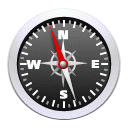
\includegraphics[width=\linewidth]{\images/chapter2/compass.png}
  	\caption{Compass sensor}
  	\label{fig:ch-2:compass}
  \end{subfigure}
  \vspace{0.00mm}
  \begin{subfigure}[b]{0.3\linewidth}
  	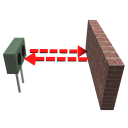
\includegraphics[width=\linewidth]{\images/chapter2/distance-sensor.png}
  	\caption{Distance sensor}
  	\label{fig:ch-2:distance-sensor}
  \end{subfigure}
  \vspace{0.00mm}
  \begin{subfigure}[b]{0.3\linewidth}
  	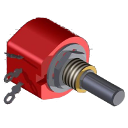
\includegraphics[width=\linewidth]{\images/chapter2/position-sensor.png}
  	\caption{Position sensor}
  	\label{fig:ch-2:position-sensor}
  \end{subfigure}
  \vspace{0.00mm}
  \caption{Sensors}
  \source{Webots documentation}
  \label{fig:ch-2:sensors}
\end{figure}

Sensors have some fields in common. For instance, the resolution field that indicates the sensitivity of the measurement. When it is set to -1 means that it will measure the infinitesimal smallest perceived change. As another example, the lookup table is a field that maps a value from the sensor read data to another custom value. Additionally, the standard deviation noise introduced by the sensor can be specified for a given measure. 

Table \ref{tab:ch-2:lookup} shows the possible values that can be associated with the lookup table field. The first column represents the data measured by the sensor, the second column is the mapped value and the third column represents the noise as a gaussian random number whose range is calculated as a percent of the response value\cite{cyberbotics}. For instance, for the row $[0.3, 50, 0.1]$ when the sensor senses an object to 0.3m of distance from the robot, it will return a value of $50 \pm 5$, where 5 represents the standard deviation, that is the $10\%$ of 50.
\begin{table}[h!]
\centering
 \begin{tabular}{c c c} 
 \hline
 Value & Mapped value & Noise \\ [0.5ex] 
 \hline\hline
 0 & 1000 & 0 \\ 
 \hline
0.1 & 1000 & 0.1 \\ 
 \hline
 0.2 & 400 & 0.1 \\ 
 \hline
 0.3 & 50 & 0.1 \\ 
 \hline
 0.37 & 30 & 0 \\ 
 \hline
\end{tabular}
\caption{Lookup table of distance sensor}
\source{Webots documentation}
\label{tab:ch-2:lookup}
\end{table}

Figure \ref{fig:ch-2:lookup} shows the relation between the current sensor values and the mapped values within the associated noise.

\begin{figure}[h!]
  \centering
  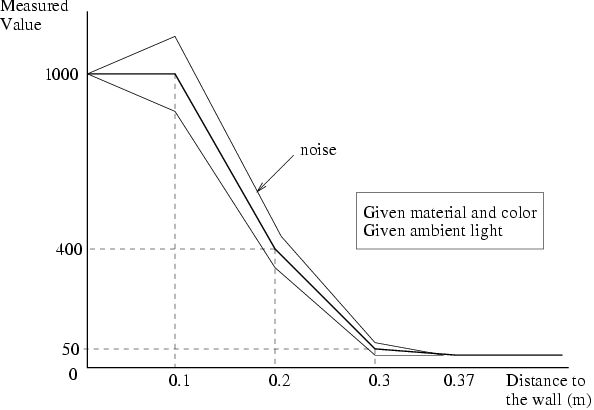
\includegraphics[width=0.8\linewidth]{\images/chapter2/lookuptable.png}
  \caption{Sensor response versus obstacle distance}
  \source{Webots documentation}
  \label{fig:ch-2:lookup}
\end{figure}

\subsection{Actuators}

Actuators allows the robot to modify the environment. Webots can simulate rotational motors, linear motors, speakers, LEDs, etc. 

\section{Probabilistic Robotics}

Robotics, according to Thrun et al.\cite{Thrun:2005:PR:1121596}, is the science of perceiving and manipulating the physical world through computer-controlled mechanical devices and it is taking place in wide areas such as medicine\cite{Azad:STAR}, planet exploration\cite{Geoffrey:venus}, agriculture\cite{Shamshiri:research-agricultural}, construction\cite{Pileun:construction}, entertainment\cite{Morris:entertainment} among others. 

The robotics that is known nowadays has being evolved across the years. From robotic systems designed to automatize highly repetitive and physically demanding human tasks in the early-to-mid-1940s\cite{Ferreira:prob}, passing through researches making the strong assumption of having exact models of robots and environments in the 1970s, to probabilistic robotics in the mid-1990s\cite{Thrun:robotic-statistics}. Thus a robot needs to deal with uncertainty most of the time. As an example, a robot that it has is ordered to walk 1 meter forward from its current position; even if it might be expected to cover that distance, due to some errors whether the robot speed was high and it slipped or the noise produced by the actuators is significant, after finishing executing the control action the robot is found in an uncertain position. That is why it needs to be capable to deal with uncertainty, predicting and preserving its current position and orientation within the environment\cite{Nikos:auxiliary-pf}.

\subsection{State}

State, according to Thrun et al.\cite{Thrun:2005:PR:1121596}, refers to the set of all aspects of the robot and its environment that can influence to the future. Two types of state can be defined:

\begin{itemize}
\item \textbf{Dynamic state} changes its position over time. For instance, the people or other robots location.
\item \textbf{Static state} does not change its position over time. For example, the walls or other moveless objects location.
\end{itemize}

Some instances of state are: 

\begin{itemize}
\item The position of physical static entities in the environment as walls, boxes, doors, etc.
\item The location and speed of mobile entities in the environment as people, other robots, etc.
\item The robot pose is usually defined by its position and its orientation relative to a global reference frame. A robot moves on a \textit{fixed frame} which is attached to the ground and does not move. This frame is called the \textit{global reference frame} (GRF). Additionally, a robot is linked within a frame which moves along with the robot. This frame is referred as \textit{local reference frame} (LRF). Communication between the coordinate frames is known as \textit{transformation of frames} and it is a key concept when modeling and programming a robot\cite{Reza:Theory-of-applied-robotics}. Figure \ref{fig:ch-2-global-local} illustrates the difference between GRF and LRF where the $X_R$ axis points to the right side of the robot, the $Y_R$ axis is aligned to its longitudinal axis and the $Z_R$ axis points upward. Besides to these Cartesian coordinates, the robot's angle orientation is defined by the Euler angles: Yaw, Pitch and Roll (see \cite{Cook:mobile-robots}). 
\end{itemize}

The notation used to represent a state at time $t$ will be denoted as $x_t$.

\begin{figure}[h!]
  \centering
  \begin{subfigure}[b]{0.5\linewidth}
  	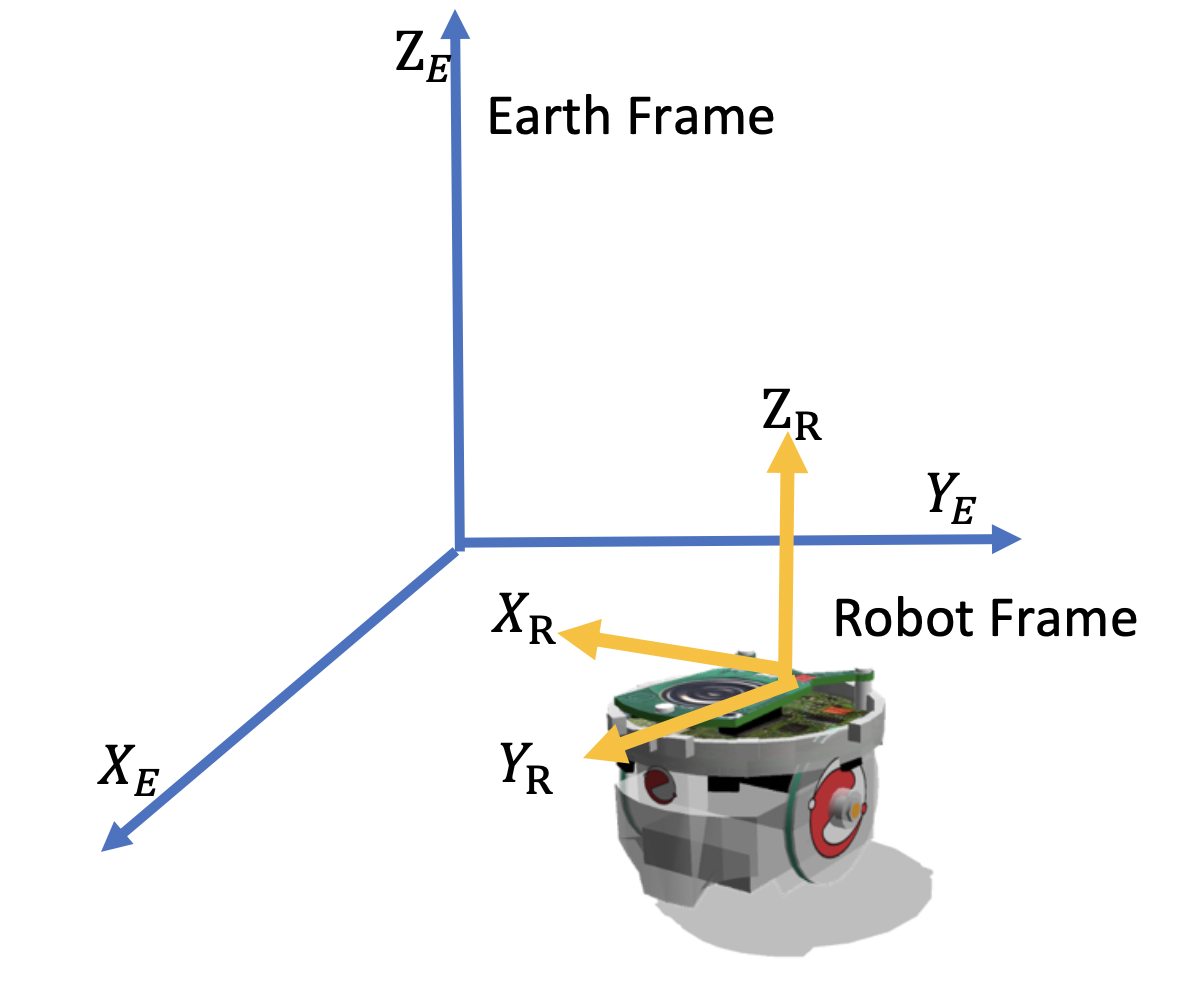
\includegraphics[width=\linewidth]{\images/chapter2/local-system.png}
  \end{subfigure}
  \caption{Local vs Global reference frame}
  \label{fig:ch-2-global-local}
\end{figure}

\subsection{Robot Versus The Environment}

A robot can interact with the environment in two ways. First, it can modify the environment state using its actuators which are drivers acting as muscles that let the robot change its configuration\cite{Reza:Theory-of-applied-robotics}. For instance, a rotational motor is an actuator that can power a joint and thus changing the robot pose. As another example, a robotic arm can be used to move objects from one position to another. Second, a robot can sense the environment using its sensors which are elements, usually attached to the robot, for obtaining information about internal and environmental states \cite{Reza:Theory-of-applied-robotics} \cite{Thrun:2005:PR:1121596}. 

The control data is information about the change of state in the environment\cite{Thrun:2005:PR:1121596}. It can be, for instance, the velocity or the acceleration of the robot at a given time $t$ and thus it will be represented as $u_t$.  The sensor data provided at time $t$ is denoted as $z_t$ and thus a sequence of sensor observations will be $z_1, z_2, ..., z_t$.

\subsection{Localisation methods}

There are two types of localisation methods categorized by the increased degree of difficulty as stated in Ferreira et al.\cite{Ferreira:prob}: 

\begin{itemize}
\item \textit{Local techniques} (also called position tracking\cite{Thrun:2005:PR:1121596}), when the robot knows its initial position and it is not able to recover if the robot loses track of it.
\item \textit{Global techniques} (see also \cite{Feng:where-am-I}), when the robot does not have any information about its initial position and it is able to estimate it even in a global uncertainty. This technique includes the \textit{kidnapped robot problem} in which a robot that knows its position is kidnapped and take it into another unknown location and its task is to recover its position. According to Thrun et al.\cite{Thrun:2005:PR:1121596} the later should be categorized as a third localisation technique given its difficulty.
\end{itemize}

Under the probabilistic approach, the robot’s momentary estimate, which represents its internal knowledge about the state of the environment (known as belief), is represented by a probability density function over the space of all locations\cite{Thrun:robotic-statistics}. That means that a robot can handle multiple ambiguous positions. After moving it can sense other factors in the environment that can lead to disambiguate its pose and put most of the probability in a single location and therefore having a better idea of where truly is. A more extensive and explicative example can be found in \cite{Thrun:robotic-statistics} and \cite{Liao:bayesian-filters} where the global localization problem is illustrated in a one-dimension space with a robot that has an hypothetical sensor that senses the presence of doors, when the robot finds the first door, the probability is distributed to all the places where there are doors (see figure \ref{fig:ch-2:sensors}). Thus the probability to be near a door is higher when the sensor detects a door but the robot does not know at this point which door is facing. Moving the robot forward makes the sensor to sense another door and thus increasing the probability of being at the second door. This illustrates some important properties of Bayes Filters that are going to be developed in more detail hereunder.

\begin{figure}[h!]
  \centering
  \begin{subfigure}[b]{\linewidth}
  	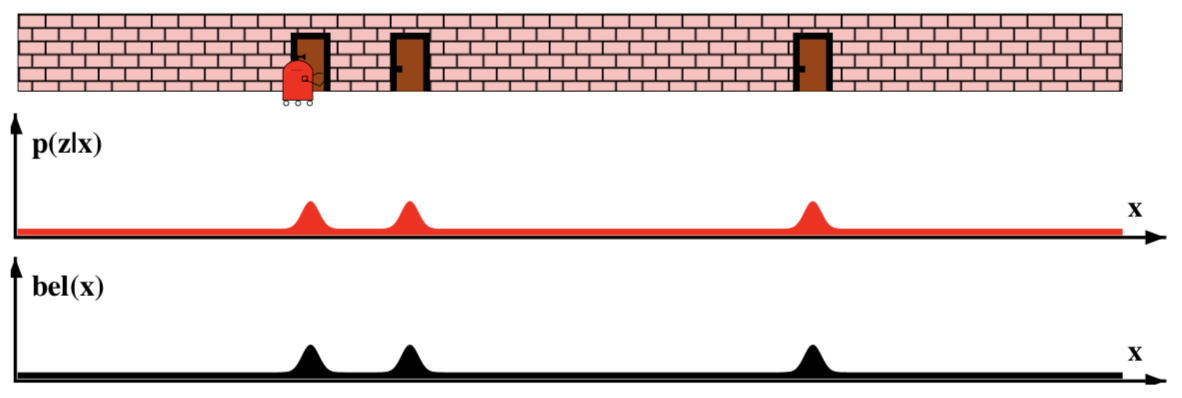
\includegraphics[width=\linewidth]{\images/chapter2/first-door.png}
  \end{subfigure}
  \vspace{1cm}
  \begin{subfigure}[b]{\linewidth}
  	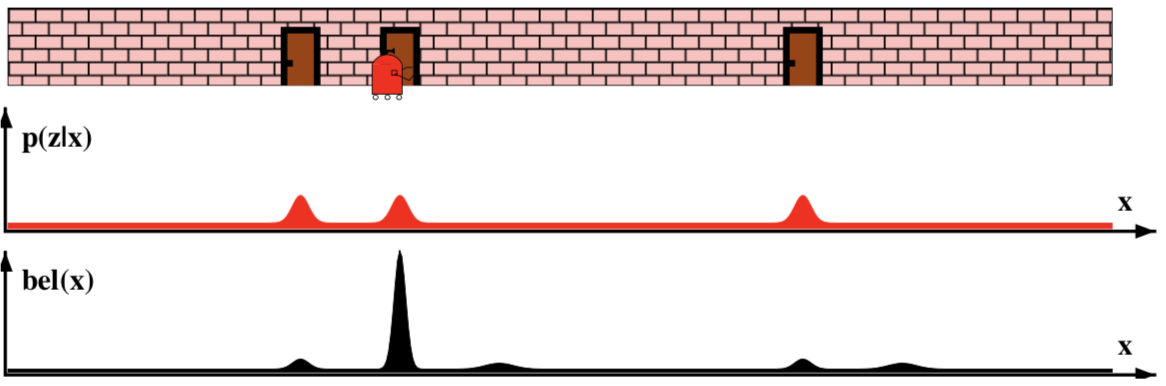
\includegraphics[width=\linewidth]{\images/chapter2/second-door.png}
  \end{subfigure}
  \caption{Probability density when robot senses.}
  \source{Extracted from Probabilistic Robotics \cite{Thrun:robotic-statistics}}
  \label{fig:ch-2:bayes-filter-example}
\end{figure}


























%\chapter{Chapter Three Title}
%\section{Section Title}
Lorem ipsum dolor sit amet, consectetur adipisicing elit, sed do eiusmod tempor incididunt ut labore et dolore magna aliqua. Ut enim ad minim veniam, quis nostrud exercitation ullamco laboris nisi ut aliquip ex ea commodo consequat. Duis aute irure dolor in reprehenderit in voluptate velit esse cillum dolore eu fugiat nulla pariatur. Excepteur sint occaecat cupidatat non proident, sunt in culpa qui officia deserunt mollit anim id est laborum.

\begin{figure}
    \centering
    \begin{subfigure}[b]{0.3\textwidth}
        \centering
        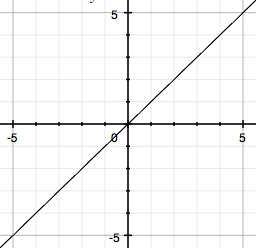
\includegraphics[width=\textwidth]{graph1}
        \caption{$y=x$}
        \label{fig:y equals x}
    \end{subfigure}
    \hfill
    \begin{subfigure}[b]{0.3\textwidth}
        \centering
        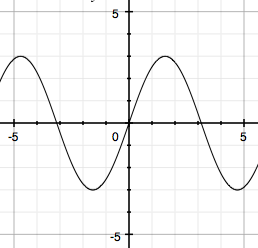
\includegraphics[width=\textwidth]{graph2}
        \caption{$y=3sinx$}
        \label{fig:three sin x}
    \end{subfigure}
    \hfill
    \begin{subfigure}[b]{0.3\textwidth}
        \centering
        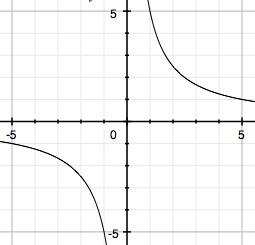
\includegraphics[width=\textwidth]{graph3}
        \caption{$y=5/x$}
        \label{fig:five over x}
    \end{subfigure}
    \caption{Three simple graphs}
    \label{fig:three graphs}
\end{figure}

Lorem ipsum dolor sit amet, consectetur adipisicing elit, sed do eiusmod tempor incididunt ut labore et dolore magna aliqua. Ut enim ad minim veniam, quis nostrud exercitation ullamco laboris nisi ut aliquip ex ea commodo consequat. Duis aute irure dolor in reprehenderit in voluptate velit esse cillum dolore eu fugiat nulla pariatur. Excepteur sint occaecat cupidatat non proident, sunt in culpa qui officia deserunt mollit anim id est laborum.

Lorem ipsum dolor sit amet, consectetur adipisicing elit, sed do eiusmod tempor incididunt ut labore et dolore magna aliqua. Ut enim ad minim veniam, quis nostrud exercitation ullamco laboris nisi ut aliquip ex ea commodo consequat. Duis aute irure dolor in reprehenderit in voluptate velit esse cillum dolore eu fugiat nulla pariatur. Excepteur sint occaecat cupidatat non proident, sunt in culpa qui officia deserunt mollit anim id est laborum.
see \ref{fig:five over x}

Lorem ipsum dolor sit amet, consectetur adipisicing elit, sed do eiusmod tempor incididunt ut labore et dolore magna aliqua. Ut enim ad minim veniam, quis nostrud exercitation ullamco laboris nisi ut aliquip ex ea commodo consequat. Duis aute irure dolor in reprehenderit in voluptate velit esse cillum dolore eu fugiat nulla pariatur. Excepteur sint occaecat cupidatat non proident, sunt in culpa qui officia deserunt mollit anim id est laborum.

\subsection{SubSection Title}
Lorem ipsum dolor sit amet, consectetur adipisicing elit, sed do eiusmod tempor incididunt ut labore et dolore magna aliqua. Ut enim ad minim veniam, quis nostrud exercitation ullamco laboris nisi ut aliquip ex ea commodo consequat. Duis aute irure dolor in reprehenderit in voluptate velit esse cillum dolore eu fugiat nulla pariatur. Excepteur sint occaecat cupidatat non proident, sunt in culpa qui officia deserunt mollit anim id est laborum.

%\chapter{Chapter Four Title}
%\section{Section Title}
Lorem ipsum dolor sit amet, consectetur adipisicing elit, sed do eiusmod tempor incididunt ut labore et dolore magna aliqua. Ut enim ad minim veniam, quis nostrud exercitation ullamco laboris nisi ut aliquip ex ea commodo consequat. Duis aute irure dolor in reprehenderit in voluptate velit esse cillum dolore eu fugiat nulla pariatur. Excepteur sint occaecat cupidatat non proident, sunt in culpa qui officia deserunt mollit anim id est laborum.

\begin{table}[h]
\centering
\begin{tabular}{l | l | l}
A & B & C \\
\hline
1 & 2 & 3 \\
4 & 5 & 6
\end{tabular}
\caption{very basic table}
\label{tab:abc}
\end{table}

Lorem ipsum dolor sit amet, consectetur adipisicing elit, sed do eiusmod tempor incididunt ut labore et dolore magna aliqua. Ut enim ad minim veniam, quis nostrud exercitation ullamco laboris nisi ut aliquip ex ea commodo consequat. Duis aute irure dolor in reprehenderit in voluptate velit esse cillum dolore eu fugiat nulla pariatur. Excepteur sint occaecat cupidatat non proident, sunt in culpa qui officia deserunt mollit anim id est laborum.

Lorem ipsum dolor sit amet, consectetur adipisicing elit, sed do eiusmod tempor incididunt ut labore et dolore magna aliqua. Ut enim ad minim veniam, quis nostrud exercitation ullamco laboris nisi ut aliquip ex ea commodo consequat. Duis aute irure dolor in reprehenderit in voluptate velit esse cillum dolore eu fugiat nulla pariatur. Excepteur sint occaecat cupidatat non proident, sunt in culpa qui officia deserunt mollit anim id est laborum.

Lorem ipsum dolor sit amet, consectetur adipisicing elit, sed do eiusmod tempor incididunt ut labore et dolore magna aliqua. Ut enim ad minim veniam, quis nostrud exercitation ullamco laboris nisi ut aliquip ex ea commodo consequat. Duis aute irure dolor in reprehenderit in voluptate velit esse cillum dolore eu fugiat nulla pariatur. Excepteur sint occaecat cupidatat non proident, sunt in culpa qui officia deserunt mollit anim id est laborum.

Lorem ipsum dolor sit amet, consectetur adipisicing elit, sed do eiusmod tempor incididunt ut labore et dolore magna aliqua. Ut enim ad minim veniam, quis nostrud exercitation ullamco laboris nisi ut aliquip ex ea commodo consequat. Duis aute irure dolor in reprehenderit in voluptate velit esse cillum dolore eu fugiat nulla pariatur. Excepteur sint occaecat cupidatat non proident, sunt in culpa qui officia deserunt mollit anim id est laborum.

\section{Section Title}
Lorem ipsum dolor sit amet, consectetur adipisicing elit, sed do eiusmod tempor incididunt ut labore et dolore magna aliqua. Ut enim ad minim veniam, quis nostrud exercitation ullamco laboris nisi ut aliquip ex ea commodo consequat. Duis aute irure dolor in reprehenderit in voluptate velit esse cillum dolore eu fugiat nulla pariatur. Excepteur sint occaecat cupidatat non proident, sunt in culpa qui officia deserunt mollit anim id est laborum.

Lorem ipsum dolor sit amet, consectetur adipisicing elit, sed do eiusmod tempor incididunt ut labore et dolore magna aliqua. Ut enim ad minim veniam, quis nostrud exercitation ullamco laboris nisi ut aliquip ex ea commodo consequat. Duis aute irure dolor in reprehenderit in voluptate velit esse cillum dolore eu fugiat nulla pariatur. Excepteur sint occaecat cupidatat non proident, sunt in culpa qui officia deserunt mollit anim id est laborum.

Lorem ipsum dolor sit amet, consectetur adipisicing elit, sed do eiusmod tempor incididunt ut labore et dolore magna aliqua. Ut enim ad minim veniam, quis nostrud exercitation ullamco laboris nisi ut aliquip ex ea commodo consequat. Duis aute irure dolor in reprehenderit in voluptate velit esse cillum dolore eu fugiat nulla pariatur. Excepteur sint occaecat cupidatat non proident, sunt in culpa qui officia deserunt mollit anim id est laborum.

\section{Section Title}
Lorem ipsum dolor sit amet, consectetur adipisicing elit, sed do eiusmod tempor incididunt ut labore et dolore magna aliqua. Ut enim ad minim veniam, quis nostrud exercitation ullamco laboris nisi ut aliquip ex ea commodo consequat. Duis aute irure dolor in reprehenderit in voluptate velit esse cillum dolore eu fugiat nulla pariatur. Excepteur sint occaecat cupidatat non proident, sunt in culpa qui officia deserunt mollit anim id est laborum.

\begin{table}[h]
    \begin{subtable}[h]{0.45\textwidth}
        \centering
        \begin{tabular}{l | l | l}
        Day & Max Temp & Min Temp \\
        \hline \hline
        Mon & 20 & 13\\
        Tue & 22 & 14\\
        Wed & 23 & 12\\
        Thurs & 25 & 13\\
        Fri & 18 & 7\\
        Sat & 15 & 13\\
        Sun & 20 & 13
        \end{tabular}
        \caption{First Week}
        \label{tab:week1}
    \end{subtable}
    \hfill
    \begin{subtable}[h]{0.45\textwidth}
        \centering
        \begin{tabular}{l | l | l}
        Day & Max Temp & Min Temp \\
        \hline \hline
        Mon & 17 & 11\\
        Tue & 16 & 10\\
        Wed & 14 & 8\\
        Thurs & 12 & 5\\
        Fri & 15 & 7\\
        Sat & 16 & 12\\
        Sun & 15 & 9
        \end{tabular}
        \caption{Second Week}
        \label{tab:week2}
    \end{subtable}
    \caption{Max and min temps recorded in the first two weeks of July}
    \label{tab:temps}
\end{table}

Lorem ipsum dolor sit amet, consectetur adipisicing elit, sed do eiusmod tempor incididunt ut labore et dolore magna aliqua. Ut enim ad minim veniam, quis nostrud exercitation ullamco laboris nisi ut aliquip ex ea commodo consequat. Duis aute irure dolor in reprehenderit in voluptate velit esse cillum dolore eu fugiat nulla pariatur. Excepteur sint occaecat cupidatat non proident, sunt in culpa qui officia deserunt mollit anim id est laborum.

Lorem ipsum dolor sit amet, consectetur adipisicing elit, sed do eiusmod tempor incididunt ut labore et dolore magna aliqua. Ut enim ad minim veniam, quis nostrud exercitation ullamco laboris nisi ut aliquip ex ea commodo consequat. Duis aute irure dolor in reprehenderit in voluptate velit esse cillum dolore eu fugiat nulla pariatur. Excepteur sint occaecat cupidatat non proident, sunt in culpa qui officia deserunt mollit anim id est laborum.

Lorem ipsum dolor sit amet, consectetur adipisicing elit, sed do eiusmod tempor incididunt ut labore et dolore magna aliqua. Ut enim ad minim veniam, quis nostrud exercitation ullamco laboris nisi ut aliquip ex ea commodo consequat. Duis aute irure dolor in reprehenderit in voluptate velit esse cillum dolore eu fugiat nulla pariatur. Excepteur sint occaecat cupidatat non proident, sunt in culpa qui officia deserunt mollit anim id est laborum.

Lorem ipsum dolor sit amet, consectetur adipisicing elit, sed do eiusmod tempor incididunt ut labore et dolore magna aliqua. Ut enim ad minim veniam, quis nostrud exercitation ullamco laboris nisi ut aliquip ex ea commodo consequat. Duis aute irure dolor in reprehenderit in voluptate velit esse cillum dolore eu fugiat nulla pariatur. Excepteur sint occaecat cupidatat non proident, sunt in culpa qui officia deserunt mollit anim id est laborum.

Lorem ipsum dolor sit amet, consectetur adipisicing elit, sed do eiusmod tempor incididunt ut labore et dolore magna aliqua. Ut enim ad minim veniam, quis nostrud exercitation ullamco laboris nisi ut aliquip ex ea commodo consequat. Duis aute irure dolor in reprehenderit in voluptate velit esse cillum dolore eu fugiat nulla pariatur. Excepteur sint occaecat cupidatat non proident, sunt in culpa qui officia deserunt mollit anim id est laborum.

Lorem ipsum dolor sit amet, consectetur adipisicing elit, sed do eiusmod tempor incididunt ut labore et dolore magna aliqua. Ut enim ad minim veniam, quis nostrud exercitation ullamco laboris nisi ut aliquip ex ea commodo consequat. Duis aute irure dolor in reprehenderit in voluptate velit esse cillum dolore eu fugiat nulla pariatur. Excepteur sint occaecat cupidatat non proident, sunt in culpa qui officia deserunt mollit anim id est laborum.

Lorem ipsum dolor sit amet, consectetur adipisicing elit, sed do eiusmod tempor incididunt ut labore et dolore magna aliqua. Ut enim ad minim veniam, quis nostrud exercitation ullamco laboris nisi ut aliquip ex ea commodo consequat. Duis aute irure dolor in reprehenderit in voluptate velit esse cillum dolore eu fugiat nulla pariatur. Excepteur sint occaecat cupidatat non proident, sunt in culpa qui officia deserunt mollit anim id est laborum.

Lorem ipsum dolor sit amet, consectetur adipisicing elit, sed do eiusmod tempor incididunt ut labore et dolore magna aliqua. Ut enim ad minim veniam, quis nostrud exercitation ullamco laboris nisi ut aliquip ex ea commodo consequat. Duis aute irure dolor in reprehenderit in voluptate velit esse cillum dolore eu fugiat nulla pariatur. Excepteur sint occaecat cupidatat non proident, sunt in culpa qui officia deserunt mollit anim id est laborum.

Lorem ipsum dolor sit amet, consectetur adipisicing elit, sed do eiusmod tempor incididunt ut labore et dolore magna aliqua. Ut enim ad minim veniam, quis nostrud exercitation ullamco laboris nisi ut aliquip ex ea commodo consequat. Duis aute irure dolor in reprehenderit in voluptate velit esse cillum dolore eu fugiat nulla pariatur. Excepteur sint occaecat cupidatat non proident, sunt in culpa qui officia deserunt mollit anim id est laborum.

%\chapter{Conclusion}
%The main purpose of this work was to present the Webots simulator and to describe the state-of-the-art regarding robot localization techniques along with Bayesian filters and finally show some preliminar results.

The present work will be used next year for the master thesis in order to implement a more generic algorithm for robot localization using more advanced techniques under the Bayesian filters literature. 



%\appendix
%\chapter{Appendix Title}
%\section{Correctness of the Bayes Filter Algorithm}\label{sec:ap:bayes-filter}
The current posterior distribution is calculated as it is shown in equation \ref{eq:ch-2:bel-derivation}.

\begin{equation}\label{eq:ch-2:bel-derivation}
p(x_t| z_{1:t}, u_{1:t}) = \frac{p(z_t | x_t, z_{1:t-1}, u_{1:t}) \: p(x_t | z_{1:t-1}, u_{1:t})}{p(z_t | z_{1:t-1}, u_{1:t})}
\end{equation}

Where,

\begin{itemize}
\item $p(x_t | z_{1:t-1}, u_{1:t})$ is the prior distribution. That is the information of state $x_t$ before seen the observation at time $t$.
\item $p(z_t | x_t, z_{1:t-1}, u_{1:t})$ is the likelihood model for the measurements. A causal, but noisy relationship\cite{Sarkka:bayesian-filters}. 
\item $p(z_t | z_{1:t-1}, u_{1:t})$ is the normalization constant defined as $\eta$
\end{itemize}

Thus equation \ref{eq:ch-2:bel-derivation} can be summarized as follows:

\begin{equation} \label{eq:ch-2:bel-derivation-2}
p(x_t| z_{1:t}, u_{1:t}) = \eta \: p(z_t | x_t, z_{1:t-1}, u_{1:t}) \: p(x_t | z_{1:t-1}, u_{1:t}) 
\end{equation}

The prediction of observation $z_t$ based on the state $x_t$, the previous observation $z_{1:t-1}$ and the control action $u_{1:t}$ has a conditional independence regarding the previous observation and the control action because they do not aport any information while predicting $z_t$. Thus the likelihood model for the measurements can be simplified as follows:

\begin{equation}
p(z_t | x_t, z_{1:t-1}, u_{1:t}) = p(z_t | x_t)
\end{equation}

Therefore equation \ref{eq:ch-2:bel-derivation-2} reduces to:

\begin{equation} \label{eq:ch-2:bel-derivation-3}
p(x_t| z_{1:t}, u_{1:t}) = \eta \: p(z_t | x_t) \: p(x_t | z_{1:t-1}, u_{1:t})
\end{equation}

In equation \ref{eq:ch-2:expand-prior-here} the prior distribution is expanded.

\begin{equation}\label{eq:ch-2:expand-prior-here}
p(x_t | z_{1:t-1}, u_{1:t}) = \int p(x_t | x_{t-1}, u_t) \: p(x_{t-1} | z_{1:t-1}, u_{1:t-1}) dx_{t-1}\\
= \overline{bel}(x_t)
\end{equation}

Replacing equation \ref{eq:ch-2:expand-prior-here} in \ref{eq:ch-2:bel-derivation-3}, equation \ref{eq:ch-2:bel-derivation-4} is obtained which is calculated by the algorithm in list \ref{ch-2:algo:bayes-filter}, third line.

\begin{equation}\label{eq:ch-2:bel-derivation-4}
p(x_t| z_{1:t}, u_{1:t}) = \eta \: p(z_t | x_t) \: \overline{bel}(x_t)
\end{equation}


\section{Correction State Algorithm in Python}\label{sec:ap:correction-state-algo}
The complete file can be found on GitHub
\footnote{\hyperref[obstacle_avoid_test.py]{https://github.com/joangerard/webots-thesis/blob/master/src}}.

\lstinputlisting[language=Python, firstline=175, lastline=211]{\code/ch-3/obstacle_avoid_test.py}






















\printbibliography

\end{document}
